\documentclass[12pt]{article}
% This first part of the file is called the PREAMBLE. It includes
% customizations and command definitions. The preamble is everything
% between \documentclass and \begin{document}.

\usepackage[margin=1in]{geometry}  % set the margins to 1in on all sides
\usepackage{graphicx}              % to include figures
\usepackage{amsmath}               % great math stuff
\usepackage{amsfonts}              % for blackboard bold, etc
\usepackage{amsthm}                % better theorem environments

\usepackage{rotating} % for sideway table
\usepackage{xcolor}
\usepackage{hyperref}
\hypersetup{
    colorlinks,
    linkcolor={red!50!black},
    citecolor={blue!50!black},
    urlcolor={blue!80!black}
}
\usepackage{cleveref}

\usepackage{array,tabularx}

\newenvironment{conditions*}
  {\par\vspace{\abovedisplayskip}\noindent
   \tabularx{\columnwidth}{>{$}l<{$} @{${}={}$} >{\raggedright\arraybackslash}X}}
  {\endtabularx\par\vspace{\belowdisplayskip}}
  
\usepackage{float}
\restylefloat{table}

% various theorems, numbered by section

\newtheorem{thm}{Theorem}[section]
\newtheorem{lem}[thm]{Lemma}
\newtheorem{prop}[thm]{Proposition}
\newtheorem{cor}[thm]{Corollary}
\newtheorem{conj}[thm]{Conjecture}

\DeclareMathOperator{\id}{id}

\newcommand{\bd}[1]{\mathbf{#1}}  % for bolding symbols
\newcommand{\RR}{\mathbb{R}}      % for Real numbers
\newcommand{\ZZ}{\mathbb{Z}}      % for Integers
\newcommand{\col}[1]{\left[\begin{matrix} #1 \end{matrix} \right]}
\newcommand{\comb}[2]{\binom{#1^2 + #2^2}{#1+#2}}

% bibliography
\usepackage{natbib}
\bibpunct{(}{)}{;}{a}{}{,} % no comma between author and year

\title{Prospectus: FDI, corruption, and the effect on private sector development}
\author{Anh Le}


\begin{document}
\maketitle

\section{Empirical Puzzle}

In recent decades, foreign direct investment (FDI) global flow has steadily increased, rising to over \$1.5 trillion dollars in 2014. For developing countries, FDI flow is also remarkably robust to global downturn, leading to enthusiastic endorsement by major international organizations as a key factor to economic development (\Cref{fig:globalfdi}).\footnote{http://www.imf.org/external/pubs/ft/fandd/1999/03/mallampa.htm, http://www.weforum.org/reports/foreign-direct-investment-key-driver-trade-growth-and-prosperity-case-multilateral-agreement} This assumption is also shared widely within political science, where much of the literature starts with the assumption that countries want to seek FDI for its many benefits. The question that these works focus on is \textit{how} countries can attract FDI, not \textit{whether} they want to do so \citep{Jensen2003, Li2003, Li2006, Ahlquist2006}.\footnote{Two recent exceptions are \citet{Pinto2013, Pandya2013}, which are the first to investigate the demand for FDI.} 

\begin{figure}[!ht]
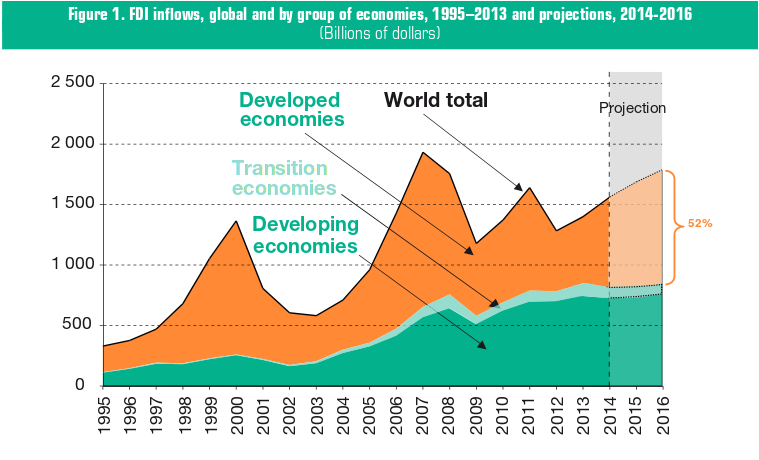
\includegraphics[width=\textwidth, height=\textheight,keepaspectratio]{../figure/global_fdi}
\caption{Source: World Investment Report, 2014}
\label{fig:globalfdi}
\end{figure}

Underlying this mode of thinking is the assumption that FDI brings various benefits to developing countries, including capital and employment. However, the most important promise that FDI holds to growth is the spillover of productivity between foreign firms and domestic firms. This can happen if local firms hire workers that were trained in a foreign firms, improve productivity through backward and forward linkages, or imitate foreign technology. According to growth theory, it is FDI's spillover, not capital or employment, that brings the technological innovation that is requisite for economic growth \citep{Findlay1978}. In this view, FDI is also a public good, providing spillover benefits to the local firms in ways that foreign firms do not take into account in their private calculations. This provides the justification for countries' using investment incentives to rectify the undersupply of FDI, closing the gap between private and social returns. 

Despite this prevailing view, there is little conclusive evidence of FDI having a positive effect on growth \citep{Nair-Reichert2001, Carkovic2002} or poverty reduction \citep{Guerra2009} (\Cref{fig:fdipoverty}). A substantial literature has developed to explain this puzzle, concluding that the growth-enhancing and spillover effect of FDI is conditional on the absorptive capacity of local firms. Cross-nationally, scholars find that FDI is more likely to have a positive growth effect when the technological gap between the local and foreign firms are small \citep{Nunnenkamp2004} and when host countries have strong financial and institutional development \citep{ Durham2004}. Similarly, absorptive capacity, measured by the level of schooling in host economy, conditions the transfer of technology between foreign and local firms across regions in China \citep{Fu2008} and countries in Latin America \citep{Willem2004}.

\begin{figure}[!ht]
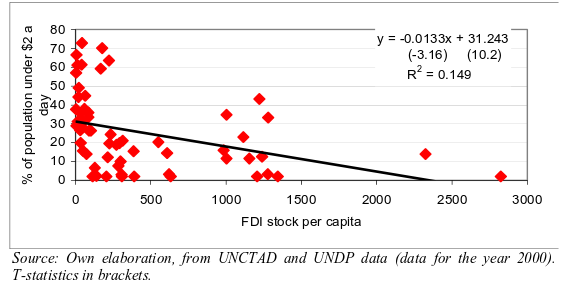
\includegraphics[width=\textwidth, height=\textheight,keepaspectratio]{../figure/fdi_poverty}
\caption{Relationship between FDI and poverty}
\label{fig:fdipoverty}
\end{figure}

Despite the resounding conclusion that the effect of FDI is highly conditional and that investment incentives do not work, why do countries still fixate so much on bringing in FDI instead of developing local absorptive capacity \citep{Blomstrom2002}? For example, Ireland provided foreign investors with lower tax rate, lower land price, and cash grants for R\&D that do not need to be repaid. China also used a tax holiday (two years of no tax and three year of half the normal tax rate) in special economic zones to attract more foreign firms \citep{Telford2001}. We see the same widespread use of investment incentives in Southeast Asia \citep{Fletcher2002}. In Vietnam, the race to offer incentives to foreign firms rages on even among sub-national units, as provincial governments defied the central government's directive and offered extra-legal incentives to FDI firms \citep{Vu2007}. Not only do these measures not work in attracting more FDI, they also deprive countries of revenues that could be spent on improving the local labor quality and investment climate, which are much more conducive to spillover effect and growth.

Thus, my dissertation project focuses on this empirical puzzle: if the positive effect of FDI is uncertain, why is there so much focus on attracting it? If developing absorptive capacity is so crucial to making FDI growth-enhancing, why is it often neglected? To understand this puzzle, I propose that we need to take into account the calculus of the individual bureaucrats and government officials, who may be more interested in the potential rents from foreign firms than the spillover and growth-enhancing effect of FDI. This is a potential reason why we often see countries (i.e. government officials) being so enthusiastic about attracting FDI, yet not so passionate about developing the local capacity that enables FDI to actually have a positive effect on growth.

\begin{figure}[!ht]
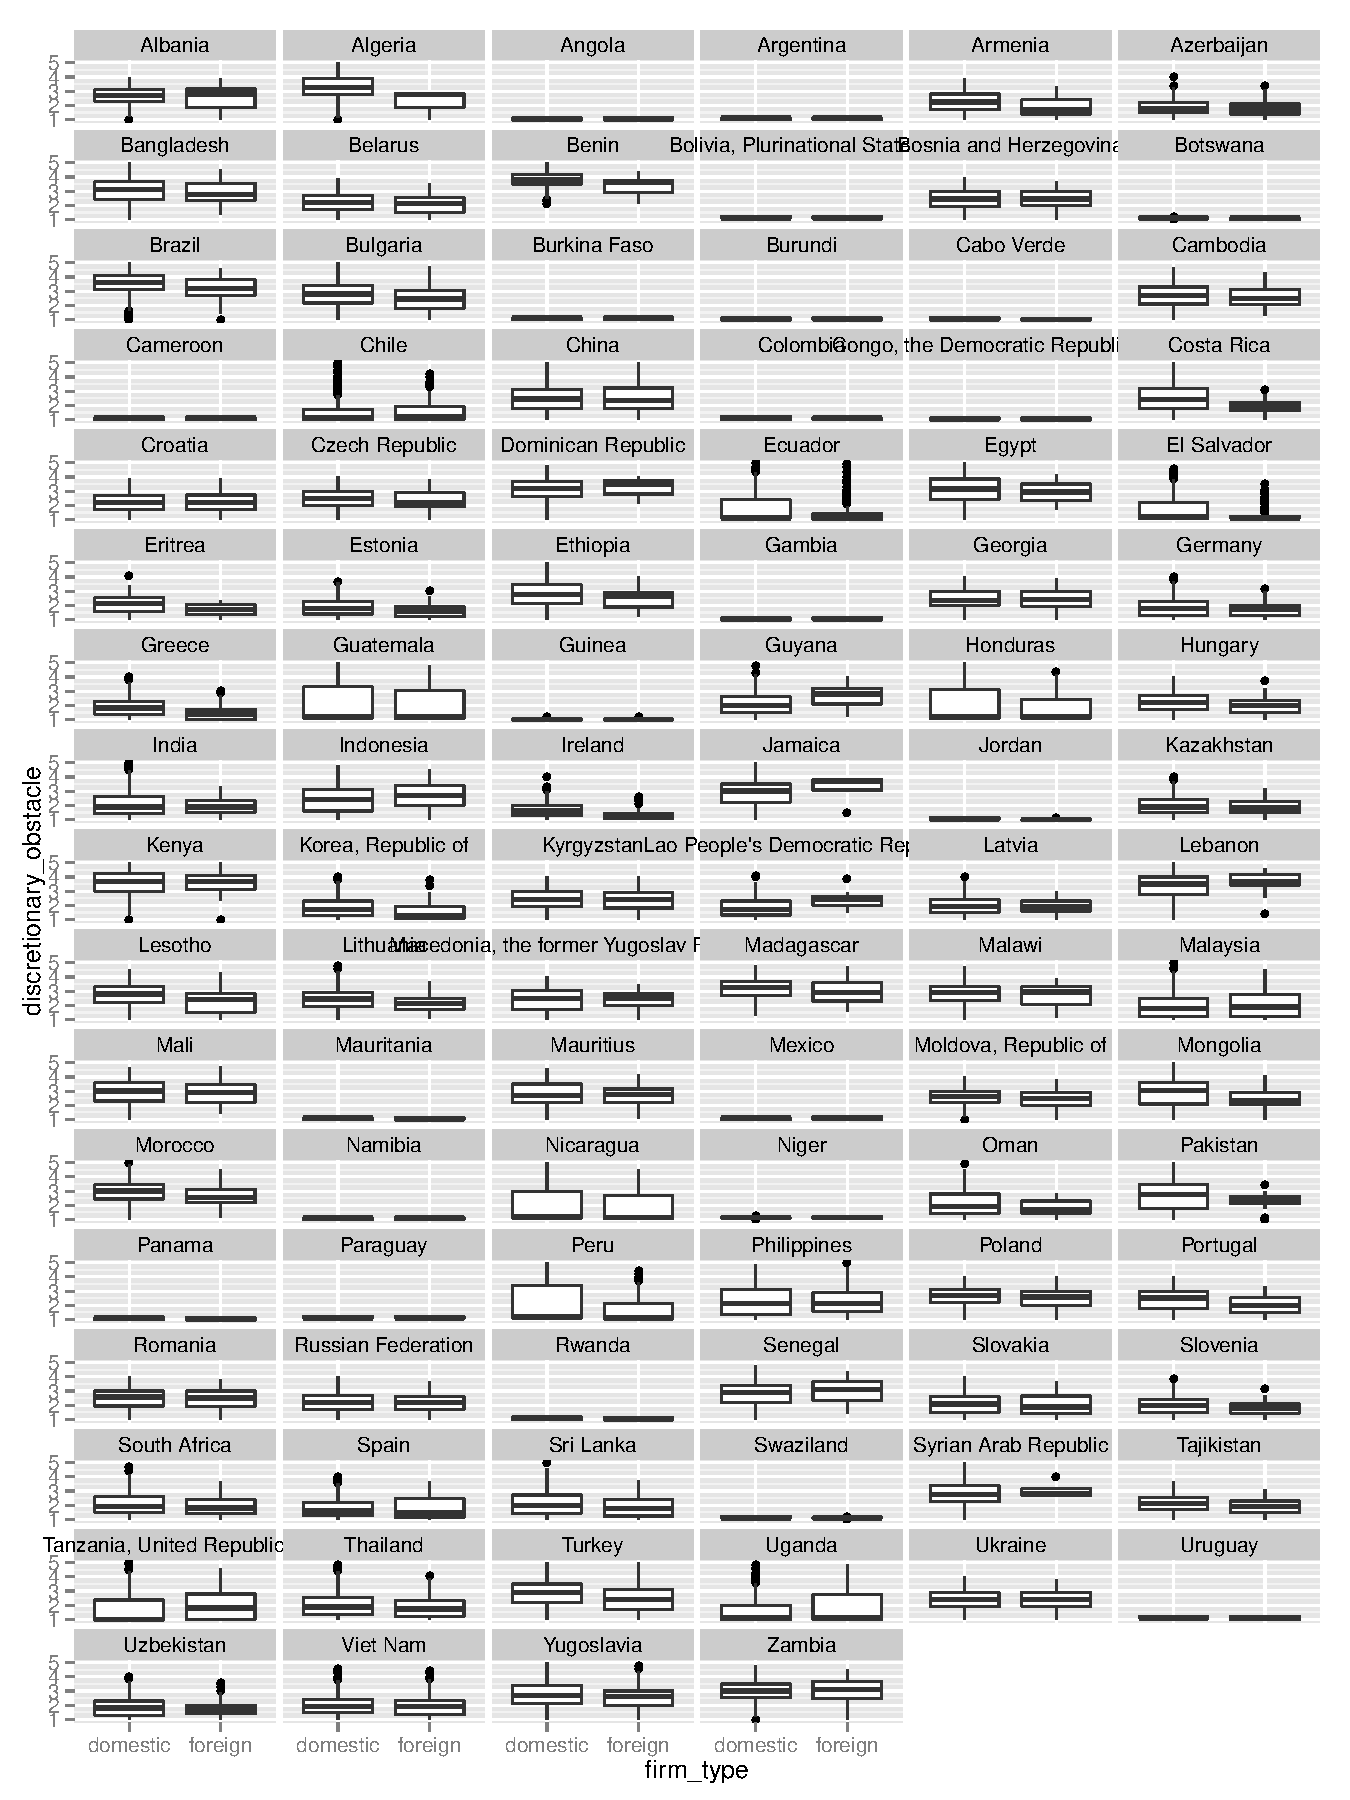
\includegraphics[width=\textwidth, height=\textheight,keepaspectratio]{../figure/fdi_domestic_treatment}
\caption{The treatment of FDI and domestic firms across countries}
\label{fig:fdi_domestic_treatment}
\end{figure}

Starting with this empirical puzzle, my project also sheds light on various related issues. First, it investigates the collusion of FDI firms and host countries' officials, a understudied phenomenon as the existing literature often assumes a foreign firm trying to fend off extortion and harassment from host countries. Second, it examines the political drivers behind private sector development, an issue whose welfare impact is well-known yet whose political determinants are ill-understood. Third, my project looks at the treatment of foreign firms versus domestic firms from a fresh angle. The majority of political science literature has considered FDI the underdog, unfamiliar with the location, susceptible to expropriation, and threatened by the lobbying effort of domestic firms. However, when FDI firms are big and resourceful, they can be an equal partner in the collusive relationship with corrupt officials to the detriment of the domestic sector.

\section{Tentative evidence}

In this section, I present some evidences that motivate the puzzle.

\begin{itemize}
	\item The spillover effect of FDI on growth is highly variable. For example, FDI is found to be growth-enhancing in East Asia, but not in Latin America \citep{Zhang2001}. Similarly, the effect of FDI on domestic investment also varies across countries and regions. FDI is found to crowd in investment in some countries (e.g. Ghana, Senegal, South Korea, Pakistan, Thailand, etc.) but crowd out in others \citep{Agosin2005}.
	
	\item Despite the prevalent concern with discrimination against foreign firms, the Wold Bank Enterprise Survey finds that foreign firms actually face fewer obstacles while doing business \citep{Batra2003}. The gap in the treatment of foreign and domestic firms also varies across countries (\Cref{fig:fdi_domestic_treatment}).
	
	\item The correlation between corruption and FDI is negative. However, there is a lot of unexplained variance at the high end of FDI. Countries with low level of FDI are always very corrupt, but countries with high level of FDI can be as well (\Cref{fig:fdi_corruption}).
	
	\begin{figure}[!ht]
	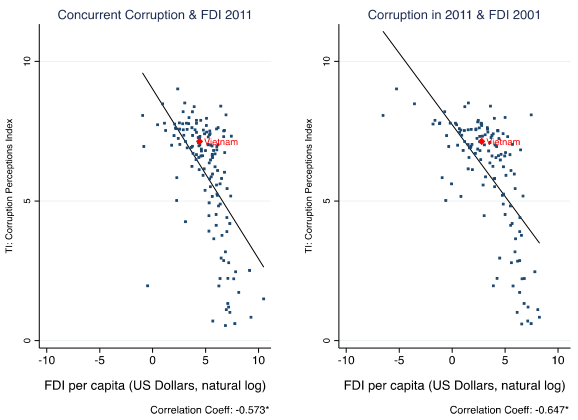
\includegraphics[width=\textwidth, height=\textheight,keepaspectratio]{../figure/fdi_corruption}
	\caption{Source: \citep{Malesky2015}}
	\label{fig:fdi_corruption}
	\end{figure}
\end{itemize}



\section{Theory}

\subsection{The spillover effect of FDI depends on government's policy to develop the domestic sector}

There are several channels through which spillover can happen, all of which require a strong domestic sector.
\begin{itemize}
	\item imitation:  domestic firms may reverse engineer a production or management technique \citep{Wang1992}. This requires 1) a small, surmountable technological gap \citep{Kokko1996}, and 2) backward linkage between local and foreign firms \citep{Javorcik2004}. Therefore, it is necessary to have technologically competent local firms that are able to supply inputs to foreign firms.
	\item skills acquisition: workers trained in foreign firms bring along their human capital when they move to domestic firms \citep{Djankov2000}. This presumes a healthy domestic sector that can offer competitive wages to workers. 
	\item competition: similar to arm's length trade, the presence of foreign firms put pressure on domestic firms to reduce inefficiency \citep{Glass2002}. For this mechanism to work, the domestic sector must survive instead of being squeezed out of market by foreign firms.
	\item export demonstration: foreign firms are more knowledgeable about exporting, which involves high fixed cost to set up a distribution and transport infrastructure, or learning about foreign taste and regulatory environment. Domestic firms can learn this ``export know-how'' from foreign firms \citep{Aitken1997}. This process, too, requires a strong domestic sector that is able to engage in commercial linkages with foreign firms.
\end{itemize}

In sum, the spillover effect of FDI depends on a strong domestic sector. Therefore, if a government is truly interested in FDI for its spillover and growth-enhancing effect, the government must be equally interested, if not more, in nurturing the absorptive capacity of domestic firms. Holding constant firm characteristics (size, sector, technological capacity, etc.), if we find that domestic firms receive worse treatment by the government, this can be evidence that the government is not primarily interested in the spillover effect of FDI.

\subsection{FDI and corruption}

My hypothesis that host country officials engage in corruption with foreign firms to the detriment of domestic firm is a novel contribution to the IPE literature of FDI and corruption. So far, the literature has been predominantly dominated by studies showing that a high level of corruption deters FDI \citep{Wei2000, Hakkala2008, Al-Sadig2009}. But what about firms that choose to invest in a highly corrupt environment nonetheless? One strain of the literature argues that foreign firms can help reduce corruption in host country via regulatory pressure effect, demonstration effect, and professionalization effect \citep{Kwok2006}; or via competing away the rents of the domestic firms, reducing the supply of bribes \citep{Sandholtz2003}. On the other hand, some argue that foreign firms, disadvantaged by their foreignness, have to bribe more and exacerbate corruption \citep{Hellman2002}.

My theory advances the literature by thinking about the behaviors of different types of foreign firms. Not all foreign firms are underdog, forced to bribe to equalize the playing field. If foreign firms enjoy regulatory privilege, they do not want to relinquish it. If foreign firms are themselves in collusion with the government, there is by definition no demonstration or professionalization effect. Indeed, foreign firms have bribed to get an upper hand in the local market\footnote{http://www.nytimes.com/2012/04/22/business/at-wal-mart-in-mexico-a-bribe-inquiry-silenced.html?pagewanted=all} or to pursue rent in protected industries \citep{Malesky2015}. In these cases, foreign firms and government officials enter a collusive relationship, resulting in the maltreatment and stunted development of domestic firms.

\begin{quote}
Hypothesis: High concentration of FDI in corrupt countries stunts the development of the domestic firms in those countries.
\end{quote}

\begin{quote}
Hypothesis: High concentration of FDI in corrupt sectors stunt the development of the domestic firms in those sectors.
\end{quote}

\subsection{Government officials and corruption}

To explain the puzzle why not all countries develop its absorptive capacity ultimately comes down to answering why some governments want growth but not others. These are big and difficult questions to study with a cross-national design due to an insurmountable degree of endogeneity. Focusing on sub-national variation, we can hold many complex political variables constant (e.g. the opportunity to seek rents, the consequence of engaging in corruption), which are often observable but hard to quantify and accounted for in quantitative analysis. Furthermore, staying within one political system, we can really delve closer to the calculus of government officials. Therefore, I develop the theory of when government officials engage in corruption with foreign firms under the context of Vietnam.

I argue that, regarding the use of FDI for rent versus for spillover, there is a principal-agent problem between the central and the provincial government. Since most FDI projects are approved at the provincial level, it is the provincial governments, not the central, that hold valuable services for sale to foreign firms. This is especially true because the implementation of law varies widely across sub-national units in Vietnam (a situation common among developing countries) \citep{Meyer2005, Thun2006}. The central government, therefore, is more removed from direct contact with FDI firms and less likely to benefit from corruption than provincial leaders. At the same time, the central government is much more concerned with overall economic growth, which is central to the longevity of the regime \citep{Malesky2008}. Therefore, the central government is more interested in the spillover effect of FDI, which necessitates the development of a strong domestic sector as discussed.  On the other hand, each provincial leader is incentivized to free-ride on the developmental effort of other provinces and of the central to keep the entire regime stable. Therefore, for provincial leaders, private rents from FDI features more heavily in the utility calculation. In contrast, central leaders care more about private sector development.

Fortunately for the central government, the principal-agent problem in this context is partially solved because monitoring is not too difficult. The central government can observe the economic performance of the provinces and use personnel management to punish and reward provincial officials \citep{Sheng2007, Li2005}.\footnote{\citet{Shih2012} recently argue that economic performance does not matter to cadre promotion. However, they investigate all members of the Chinese Central Committee, including the central party apparatus, the army, and the central economic bureaucracy. These actors are not the important decision-makers in our theory.} Therefore, the principal-agent problem is only severe when the provincial officials are not interested in further promotion to the central government. This suggests that there will be a variation in private sector development across provinces according to the provincial officials' interest in promotion. By looking at this variation in the career interest of sub-national actors, my theory contributes a fresh angle to the current literature on the relationship between decentralization and corruption, which has only postulated a one-way relationship: either decentralization increases bribery \citep{Fan2009} or reduces it \citep{Guerra2009}.

Two key assumptions in the theory above deserves further examination:
\begin{enumerate}
\item Why wouldn't Vietnam's central government worry that a developed private sector may lead to social change that undermines its position?

First, there is a large scholarship showing that authoritarian regimes are very adept at using institutions to manage regime outsiders in general and business in particular \citep{Gandhi2006, Gandhi2008, Wright2008, Le2015}. Second, if the legitimacy of the regime rests heavily on delivering economic growth, then the short-term risk of an economic downturn creating instability features much more prominently than the long-term concern with social changes. Third, it is possible to foster economic growth while restricting political freedom (e.g. Singapore). Indeed, growth can make a regime, both democratic and authoritarian, more stable, and creates room for political control \citep{Przeworski1997}.

\item Why don't provincial leaders seek rent from the domestic sector? 

First, Vietnam's private sector is still very small. It is much harder for the officials to co-ordinate and maintain secrecy when engaging in corruption with multiple domestic SMEs than with one big foreign firm. Second, growing the domestic sector big enough to seek rent is difficult. Moreover, given the rotation of officials in Vietnam, an official has few incentives to cultivate a private sector only to be rotated before reaping the benefit. Third, ironically, if officials want to grow the private sector for future rent-seeking, they must promote a enabling business environment that are free from rent-seeking. In contrast, corruption with large and existing FDI firms is much more convenient. Essentially, Vietnam's provincial officials have shifted the cost of building a thriving domestic sectors to the home countries of FDI firms and now extract rents from the high productivity and high profitability of these firms. 

\end{enumerate}


In sum, I propose a hypothesis about variation across Vietnam's provinces:

\begin{quote}
Hypothesis: High concentration of FDI in provinces where provincial leaders are not interested in promotion stunts the development of the domestic private sector
\end{quote}

\section{Research design}

\subsection{Hierarchical model using cross-national, cross-sectoral data}

To measure corruption, FDI concentration, and treatment of firms across countries, I utilize the World Bank's Enterprise Survey (ES), which includes a wealth of firm-level data across 125 countries, spanning various topics from investment, labor, to business-government relation \citep{WorldBank2015}. The Enterprise Survey uses stratified random sampling (using three strata: firm size, business sector, and region) in order to ensure representativeness. The survey data comes from face-to-face interviews with upper management and is anonymized to ensure confidentiality at all times.\footnote{For more on the methodology of the Enterprise Survey, visit \url{http://www.enterprisesurveys.org/methodology}} This dataset has a wealth of firm-level data that helps us operationalize key concepts as detailed below.

Recall our hypothesis:

\begin{quote}
Hypothesis: The presence of highly concentrated FDI in corruption countries stunts the development of the domestic private sectors
\end{quote}

\begin{quote}
Hypothesis: The presence of highly concentrated FDI in corrupt sectors stunts the development of the domestic private sectors
\end{quote}

Operationalization:
\begin{itemize}
\item FDI in countries: available via UNCTAD data on FDI flows and stocks to countries. Concentration can be measured as the ratio of FDI to GDP.
\item FDI in sectors: available via the Enterprises Survey dataset. Concentration can be measured by constructing a Herfindahl-Hirschman Index based on the size of sale, labor, or capital of firms.
\item Corruption: can be measured in two ways. 1) Firms' perception about corruption as an obstacle. This measure is frequently used but the least accurate since firms' perception of corruption depends not only on the level of corruption but also the characteristics of firms. 2) Hard measure of prevalence and depth of bribes, e.g. ``Was an informal payment expected or request (when applying for a license)?'', ``How much do establishments like this one give in informal payments?''  

\item The development of the domestic private sector: can be measured by 1) experience of domestic firms with the business environment. However, this measure may simply capture the overall governance quality instead of showing that officials have neglected domestic firms to pursue rents with FDI firms. Therefore, a better measure is 2) the gap between the experience of domestic and foreign firms. This measure is also biased against our hypothesis, since foreign firms that self-select into investing (and thus show up in our survey sample) are more similar to domestic firms than foreign firms that decide not to invest.
\end{itemize}

\subsection{Cross-sectoral and sub-national variation in Vietnam}

Despite the wealth of firm-level, cross-national data in the ES dataset, its measure of corruption is still plagued by a host of measurement issues. First, asking directly about firms' experience with corruption is unlikely to get an accurate answer due to sensitivity bias \citep{Coutts2011}. Researchers, including the ES team, often address this problem by framing the question about the experience with corruption of ``firms like yours.'' However, with this technique, firms may not read between the lines and actually answer about the experience of others \citep{Ahart2004}.

I can remedy these problems with a research design focusing on the case of Vietnam, taking advantage by a survey list experiment by \citet{Malesky2015}, which uses unmatched count technique to accurately measure the experience of firms with corruption while avoiding sensitivity bias.

Operationalization:
\begin{itemize}
\item FDI in province: Provincial statistics of FDI flow
\item FDI in sectors: PCI-FDI survey (can the survey sample be used to estimate the population's FDI?)
\item Corruption: list experiment \citep{Malesky2015}
\item Interest in promotion: 
\begin{itemize}
	\item years until retirement (retirement age is 60 for male, 55 for female)
	\item appearance in centrally controlled newspapers
\end{itemize}
\item The development of the domestic private sector:
\begin{itemize}
	\item PCI survey question: ``Do you think that the provincial officials prefer FDI?'' (Question H3)
	\item The gap in the experience of domestic and foreign firms regarding the pro-activeness of the government in helping business (Form H for domestic firms and Form J for foreign firms)
\end{itemize}
\end{itemize}

\subsection{Conjoint analysis}

While the crucial causal mechanism is the preference of provincial officials, observational data can only partially get at this because what the leaders want sometimes may not be fulfilled due to external factors (endowment, central policies). These factors can be controlled to some extent, yet the risk of mis-modeling is always present. Furthermore, what an official wants from a FDI firm is often hard to completely teased out. A big FDI firm is an attractive source of rent, but it also brings job and technology. Indeed, perhaps this high correlation is why it is so easy for officials to extract rent from FDI under the guise of promoting economic development.

To truly get at the preference of provincial leader, I plan to conduct a survey experiment using conjoint analysis to ask provincial officials about their preference between two hypothetical FDI firms \citep{Hainmueller2014}. The characteristics of these will be randomly varied across five dimensions: 1) industry, 2) size of labor force, 3) capital, 4) technology age, and 5) land, which proxies for corruption opportunities, since this is a key resource to firm that is controlled by provincial officials. If desired, it is possible to:
\begin{itemize}
\item adjust the design so that implausible hypotheticals will not appear (i.e. there should not be a high-tech company with very small capital).
\item randomize the ordering of the characteristics between respondents to test for the ordering effect (i.e. knowing a firm's industry first changes how the respondent thinks about the other characteristics)
\end{itemize}

I am mainly interested in the ``average marginal component effect'' (AMCE) of \textit{land}, which is the marginal effect of \textit{land} on the likelihood of a project being accepted, averaged over the distribution of all the other components. This allows us to back-out the what provincial officials truly want from FDI project.

\subsubsection{Experimental design}
Please read the following description carefully. Then, please indicate which project you prefer to grant investment license (cap giay phep dau tu).

\begin{center}
  \begin{tabular}{ c | c | c }
    \hline
     & Project 1 (Du an 1) & Project 2 (Du an 1) \\ \hline
    Industry &  &  \\ \hline
    Labor force &  &  \\ \hline
    Capital &  &  \\ \hline
    Land &  &  \\ \hline
    Technology age &  &  \\ \hline
    \hline
  \end{tabular}
\end{center}

If you have to choose, which project do you prefer to grant investment license? Project 1 / Project 2

\begin{itemize}
\item Industry: textile, electronics, automobile, consumer product
\item Labor force: 5, 50, 100, 200, 500 employees
\item Capital:
\item Land:
\item Technology age: 
\end{itemize}

\clearpage
\bibliographystyle{chicago}
\bibliography{library}
\end{document}
